\documentclass[11pt]{article}
\usepackage[a4paper,margin=2.4cm]{geometry}
\usepackage{amsmath,amssymb,amsthm}
\usepackage{graphicx}
\usepackage{booktabs}
\usepackage{xcolor}
\usepackage[colorlinks=true,linkcolor=blue!50!black,citecolor=blue!50!black,urlcolor=blue!50!black]{hyperref}

\newtheorem{theorem}{Theorem}
\newtheorem{proposition}{Proposition}
\newtheorem{lemma}{Lemma}
\theoremstyle{definition}
\newtheorem{hypothesis}{Hypothesis}
\newtheorem{prediction}{Prediction}
\newtheorem{problem}{Open problem}
\theoremstyle{remark}
\newtheorem{remark}{Remark}

\newcommand{\gr}{\varphi}
\newcommand{\Om}{\Omega_{\rm m}}
\newcommand{\LCDM}{$\Lambda$CDM}
\newcommand{\fede}{f_{\rm EDE}}
\newcommand{\lockdate}{19 October 2026}
\newcommand{\lockhash}{70b9cfb23fc1e0d119ebd81aed270933960fa52256f89f505f799bb3a81767f2}

\title{\textbf{Golden-Ratio Non-Resonance in Phase Space as an Organizing Hypothesis for Dark-Sector Anomalies}\\[6pt]
\large Pre-registered Predictions for the Dark-Energy Equation of State, the Growth Index and Early Dark Energy}
\author{Siddesh I. Borse\\[2pt] {\small Independent researcher}\\ {\small \href{mailto:siddesh.borase1997@gmail.com}{siddesh.borase1997@gmail.com}}\\ {\small ORCID: \href{https://orcid.org/0009-0002-3306-7175}{0009-0002-3306-7175}}}
\date{\lockdate}

\begin{document}
\maketitle

\begin{abstract}
We propose that the departures of the dark sector from \LCDM\ are set by one number, the inverse golden ratio $x = 1/\gr = (\sqrt5-1)/2$. The proposal has two strictly separated parts. The mathematical part is proven, apart from one labeled numerical result: distinct phase-space states never merge; $1/\gr$ is the global attractor of the self-similar partition $x = 1/(1+x)$ and, by Hurwitz's theorem, the most badly approximable number; and golden KAM tori are found numerically to be the most robust barriers in model four-dimensional phase spaces. The physical part is a hypothesis: dark-sector parameters take ladder values $\alpha_d x^d$, with $\alpha_d = 1$ or $\tfrac12$. Without free parameters it gives $w_0 = -\gr/2$, $w_a = -1/\gr$, a crossing of $w = -1$ at $z = 1/\sqrt5$, a growth index $\gamma = 1/\gr$ and an early-dark-energy fraction $\fede = x^4/2 = 0.073$. With DESI DR2 BAO, CMB data and four supernova samples, $(w_0, w_a) = (-0.809, -0.618)$ lies $0.3$--$1.0\sigma$ from the free fit, has the lowest AIC and BIC of the models tested, and lies at $0.5$--$1.0\sigma$ in DESI's official posteriors with supernovae. Of 403 pairs from the same algebraic family, it alone is within $1\sigma$ for all three main supernova samples. The agreement holds without CMB data and with the predicted early dark energy. Fitting $x$ freely gives $x = 0.55$--$0.69$: consistent with $1/\gr$, but neighboring values fit almost as well. The growth index is $1.1$--$1.3\sigma$ from CMB-anchored $f\sigma_8$ data. An earlier claim of $H_0 = 72.7$\,km\,s$^{-1}$\,Mpc$^{-1}$ is withdrawn, and momentum exchange is shown not to produce the predicted growth suppression. All predictions are time-stamped before any DESI data beyond DR2.
\end{abstract}

%==========================================================================
\section{Introduction}

Three observational tensions currently challenge \LCDM:
\begin{enumerate}
\item \textbf{Evolving dark energy.} DESI DR2 baryon acoustic oscillations (BAO), combined with the cosmic microwave background (CMB) and type Ia supernovae (SNe), prefer an evolving equation of state $w(a) = w_0 + w_a(1-a)$ with $w_0 > -1$ and $w_a < 0$, at $2.8$--$4.2\sigma$ depending on the SN sample~\cite{DESI-DR2}. A recalibrated DES sample (DES-Dovekie) gives a similar but weaker preference, $3.2\sigma$, with $w_0 = -0.803 \pm 0.054$ and $w_a = -0.72 \pm 0.21$ from DESI DR2, CMB (Planck, ACT and SPT) and DES-Dovekie~\cite{Dovekie}.
\item \textbf{Clustering amplitude.} Some weak-lensing surveys reported a lower $S_8$ than the CMB-anchored \LCDM\ value~\cite{DESY3}, although KiDS-Legacy finds $S_8 = 0.815$, largely consistent with the CMB~\cite{KiDSLegacy}.
\item \textbf{The Hubble tension.} The distance ladder gives $H_0 = 73.04 \pm 1.04$\,km\,s$^{-1}$\,Mpc$^{-1}$~\cite{SH0ES}, versus $67.4$\,km\,s$^{-1}$\,Mpc$^{-1}$ from the CMB~\cite{Planck2018}.
\end{enumerate}

We ask whether a single geometric principle can fix the size of these departures \emph{without free parameters}. Any such proposal faces the objection of numerology: with enough simple expressions, some will match any measurement. We address it in four ways:
\begin{enumerate}
\item We separate proven mathematics (Sec.~\ref{sec:math}) from the physical hypothesis (Sec.~\ref{sec:hyp}).
\item We quantify the look-elsewhere effect (Sec.~\ref{sec:lee}).
\item We let the data measure $x$ and compare it with other constants (Sec.~\ref{sec:freex}).
\item We time-stamp all predictions and falsification criteria before new data (Sec.~\ref{sec:prereg}).
\end{enumerate}
We also report, without omission, which earlier claims did not survive testing.

\paragraph{Related work.} The golden ratio has appeared in exact solutions of general relativity, for example in the orbits of Schwarzschild--Kottler black holes~\cite{CruzGolden} and in periodic Bianchi IX cosmologies~\cite{BryantHobill}. A search of arXiv abstracts found no previous proposal that fixes the dark-energy equation of state or the growth index by the golden ratio.

%==========================================================================
\section{Mathematical foundation}\label{sec:math}

This section collects proven results (Propositions~\ref{prop:classical}--\ref{prop:recursion}, Lemmas~\ref{lem:golden} and~\ref{lem:identities}, and the theorems of Hurwitz and KAM). It also states one well-supported but not fully general result (Remark~\ref{rem:golden}), which is labeled as such.

\subsection{Distinct states never merge in phase space}

\begin{proposition}[Classical non-intersection]\label{prop:classical}
Let $\dot{\mathbf X} = \mathbf V(\mathbf X)$ on phase space $\mathcal P \subset \mathbb R^{n}$ with $\mathbf V$ locally Lipschitz. If two solutions satisfy $\mathbf X_1(t_0) = \mathbf X_2(t_0)$ at any instant $t_0$, then $\mathbf X_1(t) = \mathbf X_2(t)$ on their common interval of existence. Distinct trajectories therefore never intersect.
\end{proposition}
\begin{proof}
Both solve the same initial-value problem, whose solution is unique by the Picard--Lindel\"of theorem~\cite{ArnoldODE}.
\end{proof}

For Hamiltonian flows, Liouville's theorem adds that phase-space volume is conserved.

\begin{proposition}[Quantum non-merging]\label{prop:quantum}
Let $U$ be unitary. For any states $|\psi\rangle, |\chi\rangle$, $\langle U\psi | U\chi\rangle = \langle\psi|\chi\rangle$. Consequently:
\begin{enumerate}
\item[(i)] orthogonal states remain orthogonal;
\item[(ii)] states with $|\langle\psi|\chi\rangle| < 1$ never evolve into the same state.
\end{enumerate}
\end{proposition}
\begin{proof}
$\langle U\psi|U\chi\rangle = \langle \psi|U^\dagger U|\chi\rangle = \langle\psi|\chi\rangle$, because $U^\dagger U = 1$.
\end{proof}

\begin{remark}
Proposition~\ref{prop:quantum} is the precise content of the intuition that ``a collision in phase space would destroy information''. It concerns distinct states; identical bosons may share a state~\cite{Sakurai}, so no universal ``no-collision'' law for particles is implied. Only the classical results are used below.
\end{remark}

\subsection{Self-similar partition and the golden ratio}

Suppose a region of phase space is partitioned into a mobile ``escape'' fraction $x$ and an excluded ``barrier'' fraction $1-x$, and that the partition is \emph{self-similar}: the barrier-to-channel ratio equals the channel-to-whole ratio.

\begin{lemma}\label{lem:golden}
The condition $(1-x)/x = x/1$ with $x > 0$ has the unique solution
\begin{equation}
x = \frac{\sqrt5 - 1}{2} = \frac1\gr \approx 0.618034, \qquad \gr = \frac{1+\sqrt5}{2}.
\end{equation}
The condition is equivalent to $x = 1/(1+x)$, so $x = [0;1,1,1,\dots]$ is the continued fraction whose partial quotients are all equal to the minimal value $1$.
\end{lemma}
\begin{proof}
$(1-x)/x = x \iff x^2 + x - 1 = 0 \iff x(1+x) = 1 \iff x = 1/(1+x)$. The positive root is $(\sqrt5-1)/2$; the other root is $-\gr$. Iterating $x = 1/(1+x)$ generates the continued fraction.
\end{proof}

\begin{proposition}[The recursive partition converges to $1/\gr$]\label{prop:recursion}
Let $f(x) = 1/(1+x)$ and $x_{n+1} = f(x_n)$ with any $x_0 \ge 0$. Then
\begin{equation}
|x_n - \gr^{-1}| \le \gr^{-n}\,|x_0 - \gr^{-1}|,
\end{equation}
so $x_n \to 1/\gr$ geometrically. For $x_0 = 1$, $x_n = F_{n+1}/F_{n+2}$ (ratios of Fibonacci numbers).
\end{proposition}
\begin{proof}
Write $x_* = 1/\gr$, which satisfies $x_* = 1/(1+x_*)$. For $x \ge 0$,
\begin{equation}
|f(x) - x_*| = \frac{|x - x_*|}{(1+x)(1+x_*)} \le \frac{|x - x_*|}{1+x_*} = x_*\,|x - x_*|.
\end{equation}
Induction gives the bound. For the Fibonacci statement, $F_{n+1}/F_{n+2} = F_{n+1}/(F_{n+1}+F_n) = 1/(1 + F_n/F_{n+1})$.
\end{proof}

So the golden ratio is not merely \emph{a} self-similar solution: it is the global attractor of the recursive partition, reached from any starting point. The map $f$ itself is not a contraction on $[0,\infty)$, since $|f'(0)| = 1$; the bound above contracts distances \emph{to the fixed point}. The two-step map $f\circ f(x) = (1+x)/(2+x)$ is a contraction on $[0,\infty)$ with constant $1/4$, so the Banach fixed-point theorem applies to it.

\subsection{Non-resonance: why $1/\gr$ is special}

\begin{theorem}[Hurwitz 1891~\cite{Hurwitz}]
For every irrational $\alpha$ there are infinitely many rationals $p/q$ with $|\alpha - p/q| < 1/(\sqrt5\, q^2)$. The constant $\sqrt5$ cannot be improved: for $\alpha = 1/\gr$ and any $c > \sqrt5$, only finitely many $p/q$ satisfy $|\alpha - p/q| < 1/(c\,q^2)$.
\end{theorem}

Numbers equivalent to $1/\gr$, that is, related to it by $\alpha \mapsto (a\alpha + b)/(c\alpha + d)$ with integers $ad - bc = \pm1$, are exactly those whose continued fraction ends in an unbroken tail of 1s (the \emph{noble} numbers). They are the \emph{most badly approximable} by rationals: they stay as far as possible from every resonance $p/q$.

\begin{theorem}[KAM, informal~\cite{Kolmogorov,Arnold63,Moser}]
In a nearly integrable Hamiltonian system with two degrees of freedom (a four-dimensional phase space) that satisfies the standard non-degeneracy condition (a twist condition for the associated area-preserving map), invariant tori whose frequency ratio is sufficiently badly approximable (Diophantine) survive sufficiently small smooth perturbations. On a three-dimensional energy surface these two-dimensional tori are impassable barriers to trajectories.
\end{theorem}

KAM theory does \emph{not} say that only golden tori survive; most sufficiently irrational tori do. Greene's residue criterion, a numerical method, and the renormalization-group analysis of MacKay indicate that in the standard map the invariant circle with golden-mean winding number is the \emph{last} to break, at $K_c \approx 0.971635$~\cite{Greene,MacKay}. Its break-up is self-similar under a renormalization operator. In phase spaces of six or more dimensions, tori no longer separate the energy surface, and trajectories can drift around them (Arnold diffusion~\cite{ArnoldDiffusion}). The barrier picture is therefore specific to two degrees of freedom.

\begin{remark}[Evidence, not a general theorem]\label{rem:golden}
Combining the results above: the winding ratio that best avoids resonance is $1/\gr$ (Hurwitz, proven). In the standard map, and conjecturally in generic area-preserving maps, the corresponding golden invariant circle is the most robust barrier (Greene, MacKay: numerical and renormalization evidence). Its self-similar structure is the fixed point of Lemma~\ref{lem:golden} and the attractor of Proposition~\ref{prop:recursion}.
\end{remark}

\subsection{Algebraic identities used below}

\begin{lemma}\label{lem:identities}
With $x = 1/\gr$:
\begin{enumerate}
\item[(a)] $x^2 = 1 - x$, $x^3 = 2x - 1 = \sqrt5 - 2$ and $x^4 = 2 - 3x$;
\item[(b)] $1 - \tfrac12 x^2 = \tfrac12(1+x) = \gr/2$;
\item[(c)] $\tfrac12 x^4 = (5 - 3\gr)/2 \approx 0.072949$;
\item[(d)] $x/(2-x) = 1/\sqrt5 = 1/(2\gr - 1)$;
\item[(e)] for any $x$, $-x - \bigl(1 + 2(-1 + \tfrac12 x^2)\bigr) = -(x^2 + x - 1)$.
\end{enumerate}
\end{lemma}
\begin{proof}
(a) From $x^2 + x - 1 = 0$; then $x^3 = x - x^2 = 2x - 1$ and $x^4 = (1-x)^2 = 2 - 3x$.
(b) $1 - \tfrac12(1-x) = \tfrac12(1+x)$, and $1 + x = \gr$.
(c) $\tfrac12(2 - 3x) = 1 - \tfrac32(\gr - 1) = (5 - 3\gr)/2$.
(d) $2 - x = \sqrt5(\sqrt5-1)/2$; and $2\gr - 1 = \sqrt5$.
(e) Direct expansion.
\end{proof}

All identities in this paper were also verified as exact symbolic identities with SymPy (see Data and code availability).

%==========================================================================
\section{The physical hypothesis}\label{sec:hyp}

Everything in this section is \emph{postulated}. Its justification is empirical (Sec.~\ref{sec:tests}), and its weak points are listed in Sec.~\ref{sec:open}.

\begin{hypothesis}[Golden non-resonance of the dark sector]\label{hyp:1}
The large-scale dynamics of the dark sector is organized like the maximally non-resonant system of Sec.~\ref{sec:math}: departures from \LCDM\ are fixed by the non-resonant fraction $x = 1/\gr$.
\end{hypothesis}

\begin{hypothesis}[Dimensional ladder]\label{hyp:2}
A dark-sector quantity that involves $d$ independent phase-space directions is set by the ladder value
\begin{equation}
\mathcal O_d = \alpha_d\, x^d, \qquad \alpha_d = \begin{cases} 1 & \text{linear or volumetric modes } (d = 1, 3),\\ \tfrac12 & \text{transverse or plasma (kinetic) modes } (d = 2, 4).\end{cases}
\end{equation}
\end{hypothesis}

\noindent The factor $x^d$ follows if the golden partition acts independently in each of $d$ directions, as a product measure. The weights $\alpha_d$ are part of the hypothesis. The value $\tfrac12$ is motivated by equipartition (one half per quadratic degree of freedom) but is not derived. The ladder values are $\mathcal O_1 = 0.618034$, $\mathcal O_2 = 0.190983$, $\mathcal O_3 = 0.236068$ and $\mathcal O_4 = 0.072949$.

\begin{hypothesis}[Assignment]\label{hyp:3}
\begin{enumerate}
\item Late-time dark energy is a transverse $d = 2$ departure: $1 + w_0 = \mathcal O_2$.
\item Structure growth is a linear $d = 1$ mode: $\gamma = \mathcal O_1$.
\item The pre-recombination early-dark-energy fraction is a plasma $d = 4$ departure: $\fede = \mathcal O_4$.
\item The evolution parameter is $w_a = -x$. Equivalently, the crossing of $w = -1$ lies at $1 - a_{\rm cross} = x/2$, so that $w_a = -(1+w_0)/(1 - a_{\rm cross}) = -x$. This is an equivalent postulate, not a derivation (Open problem~\ref{op:wa}).
\end{enumerate}
\end{hypothesis}

\noindent For dark energy and early dark energy the ladder value is the departure from \LCDM\ itself: $1 + w_0$, $w_a$ and $\fede$ all vanish in \LCDM. For growth it is the value of $\gamma$, not its shift from the general-relativity value $\gamma_{\rm GR} \simeq 0.55$; a shift-type rule is discussed in Remark~\ref{rem:alt}.

\subsection{Consequences for dark energy}

Using the Chevallier--Polarski--Linder (CPL) form $w(a) = w_0 + w_a(1-a)$~\cite{CPL1,CPL2}, a local (first-order in $1-a$) parametrization that we test below also without assuming it (Appendix~\ref{sec:binned}), and Lemma~\ref{lem:identities}:
\begin{align}
w_0 &= -1 + \tfrac12 x^2 = -\frac{\gr}{2} = -0.80902, \label{eq:w0}\\
w_a &= -x = -\frac{1}{\gr} = -0.61803, \label{eq:wa}\\
w_a &= 1 + 2 w_0, \label{eq:line}\\
1 + w_0 + w_a &= \tfrac12(1 - 3x) = -0.42705 .
\end{align}
By Lemma~\ref{lem:identities}(e), the linear relation~\eqref{eq:line} holds on the curve $(w_0, w_a) = (-1 + x^2/2, -x)$ \emph{only} at the golden value, so it is an equivalent, data-friendly statement of $x^2 + x - 1 = 0$. The dark-energy density evolves as
\begin{equation}
\frac{\rho_{\rm DE}(a)}{\rho_{\rm DE,0}} = a^{-3(1+w_0+w_a)}\, e^{-3 w_a (1-a)} = a^{\frac32(3x-1)}\, e^{3x(1-a)} .
\end{equation}
The equation of state crosses $w = -1$ where $z/(1+z) = (1+w_0)/(-w_a) = x/2$, that is,
\begin{equation}
z_{\rm cross} = \frac{x}{2-x} = \frac1{\sqrt5} = \frac{1}{2\gr - 1} = 0.44721 .
\end{equation}
At fixed redshifts the prediction is
\begin{equation}
w(z = 0.3) = -\frac{7 + 19\sqrt5}{52} = -0.9516, \qquad w(z = 0.5) = -\frac{1 + 5\sqrt5}{12} = -1.0150 .
\label{eq:fixedz}
\end{equation}

\paragraph{Physical meaning of the crossing.} Because $\mathrm d\ln\rho_{\rm DE}/\mathrm d\ln a = -3(1+w)$, the dark-energy density is \emph{maximal} exactly at $z_{\rm cross}$, about $4.75$\,Gyr ago in the best-fit background. Since then $w > -1$, so dark energy is diluting and there is no ``Big Rip''. A history with $w_0 > -1$ and $w_0 + w_a < -1$, phantom in the past and quintessence-like today, is called \emph{quintom-B}~\cite{QuintomReview}. The present values satisfy both conditions ($w_0 + w_a = -1.427$), and this is the region favored by DESI~\cite{DESI-DR2,QuintomReview}. In the same background, dark energy overtakes matter at $z = 0.334$ and acceleration begins at $z = 0.729$; neither coincides with $z_{\rm cross}$.

\paragraph{Future evolution (qualitative only).} Extrapolating the CPL form, acceleration would end when the universe is $1.67$ times its present size, and matter would dominate again at $5.2$ times. However, the same extrapolation gives $w > 1$ beyond $3.9$ times the present size, which is unphysical, so only the qualitative statement survives: in this model acceleration is a transient phase, unlike for a cosmological constant.

\subsection{Growth of structure}

Write the linear growth rate as $f(z) = \Om(z)^{\gamma}$. In general relativity (GR), $\gamma_{\rm GR} \simeq 3(1-w)/(5-6w)$ for slowly varying $w$, giving $6/11$ for $w = -1$~\cite{WangSteinhardt,Linder05}. Hypothesis~\ref{hyp:3} predicts a constant
\begin{equation}
\gamma = x = 1/\gr = 0.618 .
\end{equation}

\begin{remark}[An alternative growth rule]\label{rem:alt}
An earlier variant set $\gamma = \gamma_{\rm GR}(z) + \mathcal O_4$, a $d = 4$ shift on top of GR. In the best-fit background this gives $\gamma = 0.629, 0.620, 0.617$ at $z = 0, 0.5, 1$, numerically almost identical to $1/\gr$. The near-equality follows from the identity $\tfrac{6}{11} + \mathcal O_4 - \tfrac1\gr = \tfrac52\left(\tfrac{89}{55} - \gr\right) = 3.7\times10^{-4}$, in which $89/55$ is a Fibonacci convergent of $\gr$. That variant implies a consistency relation $\gamma - \gamma_{\rm GR} = \fede$. We adopt $\gamma = x$ because it follows the ladder assignment (growth is a linear, $d = 1$ mode); current data cannot distinguish the two forms ($\chi^2 = 8.13$ versus $8.19$, Sec.~\ref{sec:growth}).
\end{remark}

\subsection{Embedding in standard frameworks}\label{sec:embed}

The ladder fixes numbers, not dynamics. To make the predictions computable and comparable with published constraints, we embed each of them in an established effective framework.

\paragraph{Phantom crossing: parametrized post-Friedmann dark energy.} A single canonical scalar field cannot cross $w = -1$~\cite{Vikman}. The standard remedy, used by DESI whenever $w$ crosses $-1$~\cite{DESI-DR2}, is the parametrized post-Friedmann (PPF) description~\cite{FangHuLewis}. It treats dark energy as an effective component whose perturbations remain stable through the crossing. Prediction~\ref{pred:de} is a statement about this effective $w(a)$.

\paragraph{Growth: effective gravitational coupling.} In the quasi-static regime, phenomenological modified gravity multiplies the source of matter clustering by $\mu(a)$~\cite{AKS}. With $N = \ln a$ and $f = \mathrm d\ln\delta/\mathrm dN$,
\begin{equation}
f' + f^2 + \left(2 + \frac{\mathrm d\ln H}{\mathrm dN}\right) f = \frac32\,\mu(a)\,\Om(a).
\label{eq:mu}
\end{equation}
Inserting $f = \Om^{1/\gr}$ in the best-fit $\gr$-ladder background gives $\mu - 1 = -0.178$, $-0.125$, $-0.068$ and $-0.020$ at $z = 0$, $0.5$, $1$ and $2$. This is described to within $0.018$ (for $z < 3$) by the time dependence used in the DESI modified-gravity analyses~\cite{Ishak},
\begin{equation}
\mu(a) = 1 + \mu_0\,\frac{\Omega_{\rm DE}(a)}{\Omega_{\rm DE,0}}, \qquad \mu_0 \simeq -0.20 .
\end{equation}
Gravity acting on matter clustering is weakened by about a fifth today, fading as dark energy becomes subdominant. The lensing response $\Sigma$ is not fixed by the ladder (Open problem~\ref{op:mech}).

\paragraph{Early dark energy.} Prediction~\ref{pred:ede} refers to the axion-like early dark energy of Poulin et al.~\cite{Poulin}, with potential $V(\phi) \propto [1 - \cos(\phi/f_a)]^3$ (here $\phi$ is the EDE field, not the golden ratio $\gr$) and peak fraction $\fede$ at the critical redshift $z_c$.

%==========================================================================
\section{Tests against current data}\label{sec:tests}

All code, data products and outputs are public (see Data and code availability).

\subsection{Data and method}

\begin{itemize}
\item \textbf{BAO.} 13 DESI DR2 measurements of $D_V/r_d$, $D_M/r_d$ and $D_H/r_d$, with the full covariance~\cite{DESI-DR2}.
\item \textbf{CMB.} Planck 2018 distance priors $(R, \ell_A, \omega_b)$ with their correlation matrix~\cite{ChenHuangWang,Planck2018}, and, separately, DESI's official Markov chains computed with the full CMB likelihoods~\cite{DESIchains}.
\item \textbf{SNe.} Pantheon+ (1590 light curves with $z > 0.01$)~\cite{PantheonPlus}, Union3 (22 binned magnitudes)~\cite{Union3}, DESY5 (1829 SNe)~\cite{DESY5} and the recalibrated DES-Dovekie (1820 SNe)~\cite{Dovekie}, each with its full statistical and systematic covariance. The absolute magnitude is marginalized analytically:
\begin{equation}
\chi^2_{\rm SN} = \mathbf r^{\rm T} C^{-1}\mathbf r - \frac{(\mathbf 1^{\rm T}C^{-1}\mathbf r)^2}{\mathbf 1^{\rm T} C^{-1}\mathbf 1}.
\end{equation}
\item \textbf{Theory.} A flat universe with photons, $N_{\rm eff} = 3.046$, and one massive neutrino of $0.06$\,eV carrying $N_{\rm eff}/3$. The massive-neutrino density uses the fitting formula of Komatsu et al.~\cite{Komatsu} at all redshifts. The drag scale uses the DESI calibrated fit~\cite{DESI-Y1},
\begin{equation}
r_d = 147.05\,\mathrm{Mpc}\,\left(\frac{\omega_b}{0.02236}\right)^{-0.13}\left(\frac{\omega_{m}}{0.1432}\right)^{-0.23}\left(\frac{N_{\rm eff}}{3.04}\right)^{-0.1}.
\end{equation}
The distance priors of Ref.~\cite{ChenHuangWang} were built with the decoupling redshift $z_*$ of the Planck chains. We therefore use the Hu--Sugiyama fit~\cite{HuSugiyama} times a quadratic correction calibrated against CAMB~\cite{CAMB}, with residuals below $4\times10^{-7}$.
\item \textbf{Validation against Planck and CAMB.} For Planck 2018 parameters our code gives $r_s(z_*) = 144.43$\,Mpc, $r_d = 147.09$\,Mpc and $100\theta_* = 1.04110$, identical to the Planck values. For the $\gr$-ladder best fit it agrees with CAMB to $0.001\%$ in $H(z)$ and $D_M(z)$, $0.001\%$ in $R$, $0.002\%$ in $\ell_A$, $0.03\%$ in $r_d$ (the accuracy of the DESI fit), and $0.23\%$ in the shape of $f\sigma_8(z)$ up to $z = 2$.
\item \textbf{Models.}
  \begin{itemize}
  \item \LCDM;
  \item the hypothesis (``$\gr$-ladder'', Eqs.~\eqref{eq:w0}--\eqref{eq:wa});
  \item the alternative $d = 3$ branch, $1 + w_0 = x^3$;
  \item $w_0w_a$CDM.
  \end{itemize}
  All share the parameters $(\omega_{bc}, \omega_b, h)$; $w_0w_a$CDM adds two.
\end{itemize}

\subsection{Late-time dark energy}

\begin{table}[t]
\centering
\small
\begin{tabular}{llrrrrr}
\toprule
Data & Model & $\chi^2_{\min}$ & $\chi^2/{\rm dof}$ & AIC & BIC & $n\sigma$ vs.\ free \\
\midrule
DESI+CMB & \LCDM & 14.64 & 1.126 & 20.64 & 22.96 & 2.31 \\
 & $\gr$-ladder & 9.36 & 0.720 & \textbf{15.36} & \textbf{17.67} & 1.04 \\
 & $w_0w_a$ & 6.92 & 0.629 & 16.92 & 20.78 & -- \\
\midrule
+Pantheon+ & \LCDM & 1420.40 & 0.887 & 1426.40 & 1442.55 & 2.24 \\
 & $\gr$-ladder & 1414.03 & 0.883 & \textbf{1420.03} & \textbf{1436.18} & 0.51 \\
 & $w_0w_a$ & 1413.04 & 0.883 & 1423.04 & 1449.94 & -- \\
\midrule
+Union3 & \LCDM & 43.05 & 1.266 & 49.05 & 53.96 & 3.25 \\
 & $\gr$-ladder & 31.40 & 0.923 & \textbf{37.40} & \textbf{42.31} & 0.85 \\
 & $w_0w_a$ & 29.53 & 0.923 & 39.53 & 47.71 & -- \\
\midrule
+DESY5 & \LCDM & 1664.06 & 0.904 & 1670.06 & 1686.62 & 3.80 \\
 & $\gr$-ladder & 1646.88 & 0.895 & \textbf{1652.88} & \textbf{1669.44} & 0.28 \\
 & $w_0w_a$ & 1646.38 & 0.895 & 1656.38 & 1683.98 & -- \\
\midrule
+DES-Dovekie & \LCDM & 1649.71 & 0.900 & 1655.71 & 1672.26 & 2.80 \\
 & $\gr$-ladder & 1639.71 & 0.895 & \textbf{1645.71} & \textbf{1662.25} & 0.30 \\
 & $w_0w_a$ & 1639.17 & 0.896 & 1649.17 & 1676.75 & -- \\
\bottomrule
\end{tabular}
\caption{Model comparison with compressed CMB information. The last column converts $\chi^2 - \chi^2_{w_0w_a}$ (2 degrees of freedom) into Gaussian $\sigma$. The $\gr$-ladder has no free dark-energy parameters and the lowest AIC and BIC in every combination. Degrees of freedom subtract one per SN sample for the marginalized magnitude; $\chi^2/{\rm dof} < 1$ for the large SN samples reflects their conservative error budgets. The $d = 3$ branch is $1.0$--$2.2\sigma$ from the free fit.}
\label{tab:fits}
\end{table}

Table~\ref{tab:fits} and Fig.~\ref{fig:w0wa} summarize the results. The $\gr$-ladder lies $0.3$--$1.0\sigma$ from the free fit and is preferred over \LCDM\ by $\Delta\chi^2 = 5.3$--$17.2$. In the same fits, \LCDM\ is disfavored at $2.2$--$3.8\sigma$, close to the published DESI values ($2.8$--$4.2\sigma$, full CMB); the difference comes from using compressed CMB information. With DES-Dovekie the free best fit is $(w_0, w_a) = (-0.822, -0.637)$, within $0.02$ of the prediction. The DES-Dovekie analysis itself, with full CMB likelihoods, finds $w_0 = -0.803 \pm 0.054$ and $w_a = -0.72 \pm 0.21$~\cite{Dovekie}; the prediction lies $0.1\sigma$ and $0.5\sigma$ from these values, one parameter at a time (no correlation coefficient is quoted, so we give no joint level). The best-fit $\gr$-ladder backgrounds have $H_0 \simeq 67.1$--$67.2$\,km\,s$^{-1}$\,Mpc$^{-1}$ and $\Om \simeq 0.316$--$0.317$.

\begin{figure}[t]
\centering
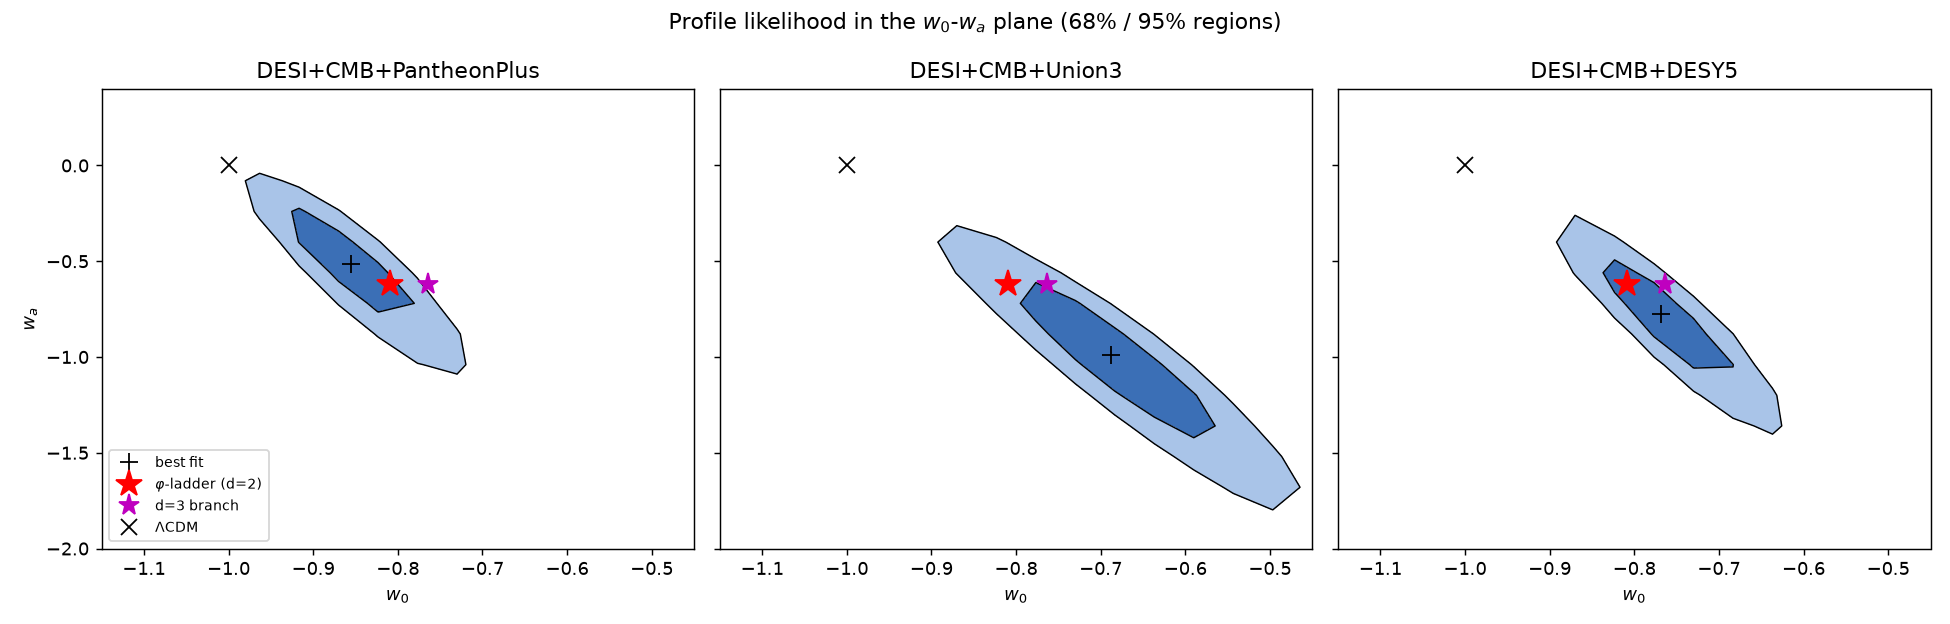
\includegraphics[width=\textwidth]{figures/fig4_w0wa_likelihood.png}
\caption{Profile likelihood in the $w_0$--$w_a$ plane (68\% and 95\% regions) for DESI DR2 BAO + CMB distance priors + each SN sample. Red star: $\gr$-ladder prediction. Magenta star: $d = 3$ branch. Cross: \LCDM.}
\label{fig:w0wa}
\end{figure}

\subsection{Official DESI posteriors with the full CMB likelihood}\label{sec:official}

The DESI collaboration has released its DR2 Markov chains~\cite{DESIchains}. The paper's default CMB combination is:
\begin{itemize}
\item Planck PR3 low-$\ell$ TT and EE;
\item Planck PR4 CamSpec high-$\ell$ TT, TE and EE;
\item Planck PR4 and ACT DR6 lensing.
\end{itemize}
After discarding the first 30\% of each chain as burn-in, we build a smoothed, weighted 2D histogram of $(w_0, w_a)$. A point's credible level is the posterior mass in regions of higher density, i.e.\ the contour through it, converted to a two-sided Gaussian $\sigma$. Our posterior means reproduce the published DESI values to the quoted precision. For DESI+CMB+Pantheon+, for example, we find $w_0 = -0.838 \pm 0.055$ and $w_a = -0.617 \pm 0.208$, against the published $-0.838 \pm 0.055$ and $-0.62^{+0.22}_{-0.19}$ (DESI quotes asymmetric 68\% intervals for $w_a$)~\cite{DESI-DR2}.

\begin{table}[t]
\centering
\small
\begin{tabular}{lccc}
\toprule
Official DESI DR2 chains & $\gr$-ladder level & $n\sigma$ & \LCDM\ (DESI) \\
\midrule
DESI+CMB (baseline) & 85.3\% & 1.45 & $3.1\sigma$ \\
+Pantheon+ & 39.9\% & 0.52 & $2.8\sigma$ \\
+Union3 & 70.4\% & 1.04 & $3.8\sigma$ \\
+DESY5 & 40.4\% & 0.53 & $4.2\sigma$ \\
\midrule
DESI+CMB, Planck PR3 plik & 80.2\% & 1.29 & \\
+DESY5, Planck PR3 plik & 35.8\% & 0.47 & \\
+DESY5, HiLLiPoP/LoLLiPoP & 21.1\% & 0.27 & \\
+DESY5 with $z > 0.1$ & 17.8\% & 0.23 & \\
DESI BAO only (no CMB) & 72.2\% & 1.08 & \\
DESI BAO + DESY5 (no CMB) & 10.7\% & 0.14 & \\
\bottomrule
\end{tabular}
\caption{Position of $(-\gr/2, -1/\gr)$ in the official DESI DR2 $w_0w_a$CDM posteriors. The upper block is DESI's baseline; the lower block replaces the CMB likelihood, cuts low-redshift SNe, or drops the CMB entirely. The last column quotes DESI's own preference against \LCDM~\cite{DESI-DR2}. The $d = 3$ branch lies at $1.7$, $2.6$, $1.4$ and $1.6\sigma$ in the baseline chains. The non-crossing history of Appendix~\ref{sec:drag} lies outside the sampled region in every combination; a Gaussian estimate gives $4.0$--$5.3\sigma$.}
\label{tab:official}
\end{table}

The prediction lies at $0.5\sigma$ (Pantheon+, DESY5) and $1.0\sigma$ (Union3) with supernovae, and at $1.45\sigma$ for DESI+CMB alone. It is equally consistent with alternative CMB likelihoods ($0.27$--$1.29\sigma$), with a low-redshift SN cut ($0.23\sigma$), and without any CMB data ($0.14$--$1.08\sigma$), so the agreement is not driven by one dataset choice (Table~\ref{tab:official}, Fig.~\ref{fig:official}).

\begin{figure}[t]
\centering
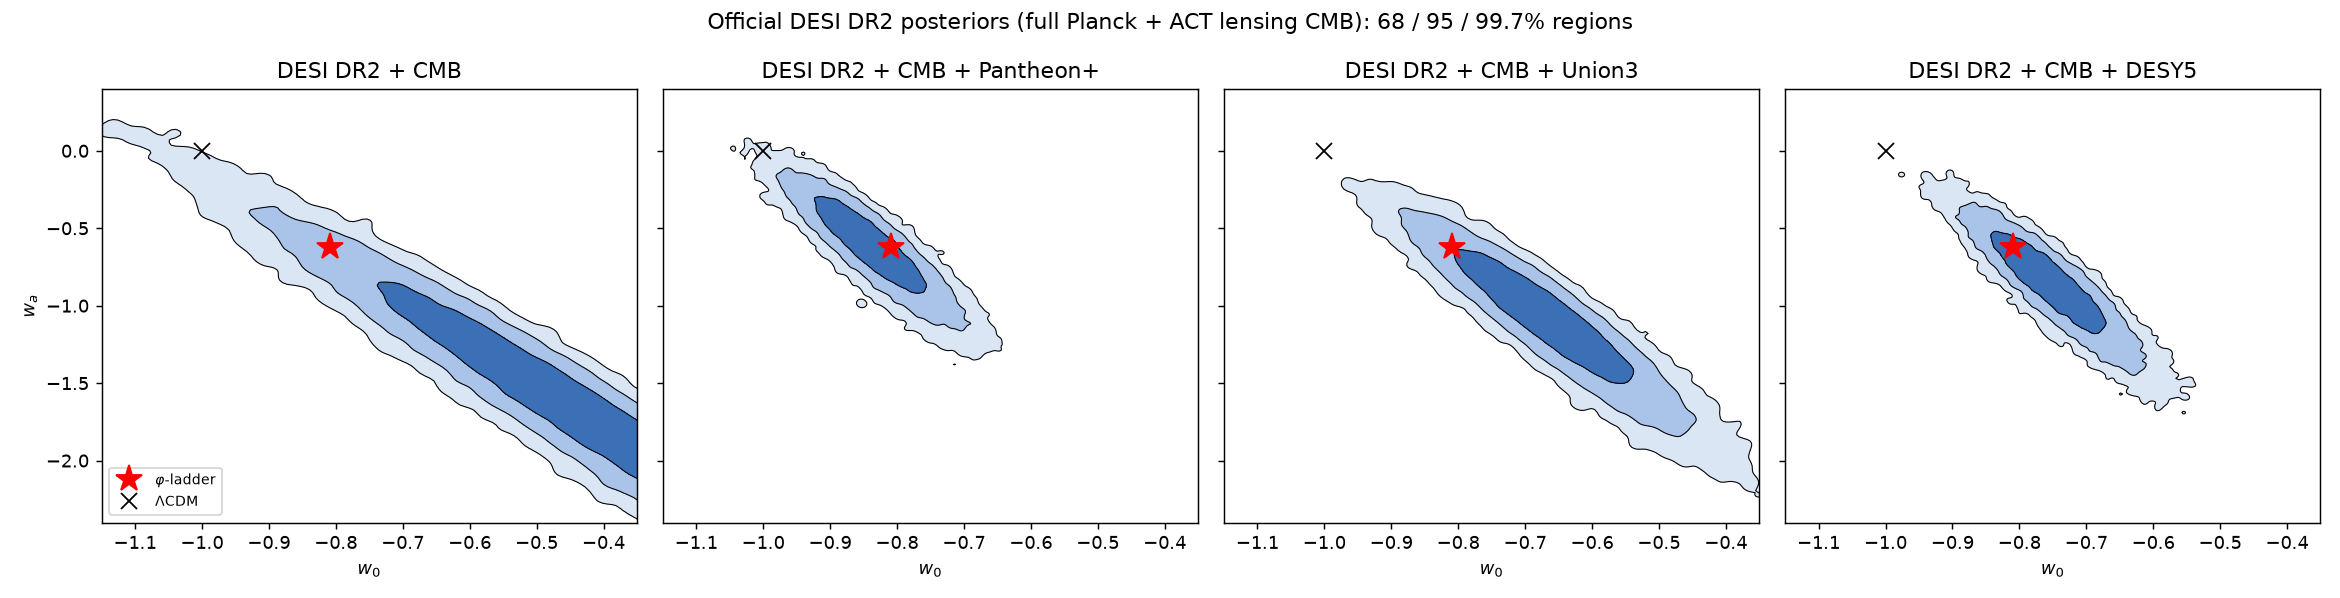
\includegraphics[width=\textwidth]{figures/fig8_desi_official_chains.png}
\caption{Official DESI DR2 $w_0w_a$CDM posteriors with the full Planck CMB likelihood and Planck + ACT lensing (68, 95 and 99.7\% regions). Red star: $\gr$-ladder prediction. Cross: \LCDM.}
\label{fig:official}
\end{figure}

\subsection{The best-measured redshift (pivot) and fixed-redshift tests}\label{sec:pivot}

DESI constrains $w$ most precisely at a pivot redshift $z_p$, where $w$ is uncorrelated with $w_a$. Table~\ref{tab:pivot} compares the prediction at each pivot and at the fixed redshifts of Eq.~\eqref{eq:fixedz}. At the pivot the prediction agrees to $0.00$--$1.16\sigma$. The predicted crossing, $z = 0.447$, lies inside the range of pivot redshifts ($0.31$--$0.53$), so the theory, like the data, has $w_p$ close to $-1$ at the best-measured redshift even though $w_0$ and $w_a$ both differ from their \LCDM\ values. This test uses the same chains as Table~\ref{tab:official}, so it is a sharper presentation rather than independent evidence.

\begin{table}[t]
\centering
\small
\begin{tabular}{lcccccc}
\toprule
Chains & $z_p$ & $w_p$ (DESI) & $w_p$ (theory) & dev. & $w(0.3)$: dev. & $w(0.5)$: dev. \\
\midrule
DESI+CMB & 0.53 & $-1.024 \pm 0.043$ & $-1.023$ & $0.02\sigma$ & $-1.63\sigma$ & $-0.31\sigma$ \\
+Pantheon+ & 0.31 & $-0.984 \pm 0.025$ & $-0.956$ & $1.16\sigma$ & $1.16\sigma$ & $0.90\sigma$ \\
+Union3 & 0.39 & $-0.972 \pm 0.032$ & $-0.983$ & $-0.33\sigma$ & $-0.98\sigma$ & $0.39\sigma$ \\
+DESY5 & 0.31 & $-0.954 \pm 0.024$ & $-0.954$ & $0.00\sigma$ & $-0.04\sigma$ & $0.73\sigma$ \\
\bottomrule
\end{tabular}
\caption{Pivot and fixed-redshift tests in the official DESI chains. ``dev.'' is $(\text{theory} - \text{DESI})/\sigma$. The theory gives $w(0.3) = -0.9516$ and $w(0.5) = -1.0150$.}
\label{tab:pivot}
\end{table}

\subsection{Robustness of the dark-energy result}\label{sec:robust}

Two further tests, detailed in the appendices, check that the agreement is not an artifact of the CPL form or of the assumed early-universe physics:
\begin{itemize}
\item \textbf{Shape of $w(z)$ (Appendix~\ref{sec:binned}).} Against DESI's model-independent binned reconstruction, the predicted $w(z)$ deviates by $1.0$--$1.75\sigma$, comparable to DESI's own best-fit CPL models ($0.3$--$1.5\sigma$).
\item \textbf{Early-universe physics (Appendix~\ref{sec:joint}).} Without CMB data and with $r_d$ free, the $\gr$-ladder lies $0.1$--$1.1\sigma$ from the free fit; with CMB data and the predicted early dark energy included, it lies $0.2$--$1.3\sigma$ from it.
\end{itemize}

\subsection{Letting the data measure $x$}\label{sec:freex}

We fit the one-parameter curve $(w_0, w_a) = (-1 + x^2/2, -x)$ with $x$ free (Fig.~\ref{fig:freex}). The data prefer the following values:

\begin{center}
\small
\begin{tabular}{lcc}
\toprule
Data & best $x$ & 68\% range \\
\midrule
DESI+CMB & 0.692 & [0.54, 0.80] \\
+Pantheon+ & 0.550 & [0.46, 0.62] \\
+Union3 & 0.692 & [0.61, 0.77] \\
+DESY5 & 0.643 & [0.58, 0.70] \\
+DES-Dovekie & 0.576 & [0.50, 0.64] \\
\bottomrule
\end{tabular}
\end{center}

The density of the official chains along the same curve gives consistent values ($0.555$--$0.695$). The five 68\% ranges overlap only in $[0.61, 0.62]$, which contains $1/\gr = 0.618$. Among nine simple constants ($1/e$, $0.5$, $0.6$, $1/\gr$, $\pi/5$, $2/3$, $\ln 2$, $1/\sqrt2$, $0.75$), $1/\gr$ is the only one inside every 68\% range. It is, however, at the edge for Pantheon+ ($\Delta\chi^2 = 0.98$), and the nearby values $0.6$ and $\pi/5$ miss only narrowly. The datasets share BAO and CMB information, so these ranges are not independent.

\textbf{Conclusion:} current data measure $x \approx 0.55$--$0.69$ and are fully consistent with $1/\gr$, but they \emph{cannot single out} $\gr$ from its neighbors. That is why the predictions are pre-registered.

\begin{figure}[t]
\centering
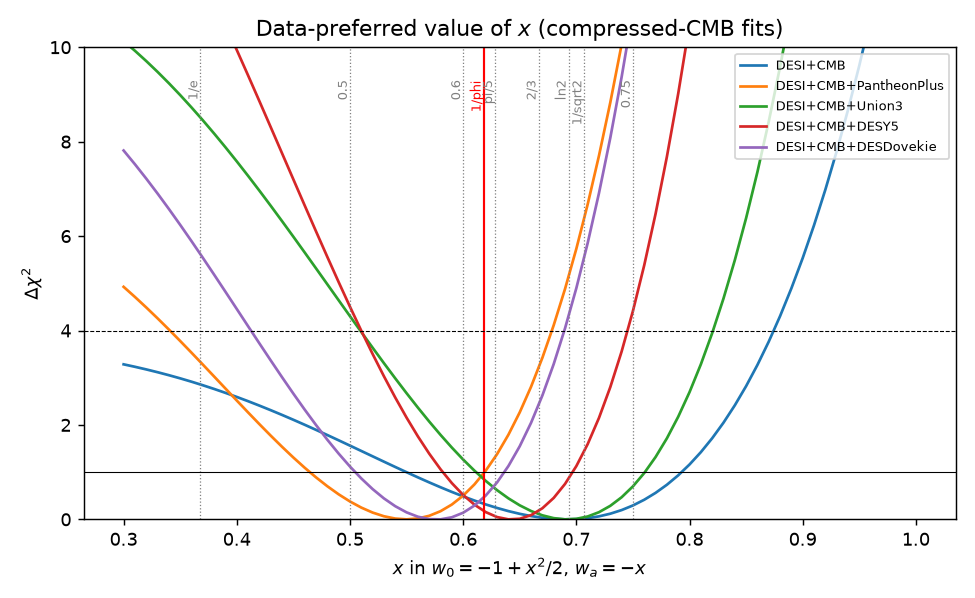
\includegraphics[width=0.78\textwidth]{figures/fig9_x_profile.png}
\caption{$\Delta\chi^2$ as a function of $x$ on the ladder curve, for each data combination. Vertical lines mark simple constants; red marks $1/\gr$. Horizontal lines: $\Delta\chi^2 = 1$ and $4$.}
\label{fig:freex}
\end{figure}

\subsection{Bayes factors}\label{sec:bayes}

For a point nested in $w_0w_a$CDM, the Savage--Dickey ratio gives the Bayes factor directly as the posterior density at the point divided by the prior density. We use DESI's priors~\cite{DESI-DR2}: $w_0 \in U[-3, 1]$, $w_a \in U[-3, 2]$ and $w_0 + w_a < 0$, a prior area of $15.5$. From the official chains, varying the histogram smoothing:
\begin{itemize}
\item \textbf{The $\gr$ point versus free $(w_0, w_a)$:} $B = 14$--$16$ (DESI+CMB), $270$--$280$ (+Pantheon+), $67$--$77$ (+Union3) and $250$--$270$ (+DESY5), so the fixed point is strongly favored over the two-parameter extension.
\item \textbf{\LCDM\ versus free $(w_0, w_a)$:} $B = 0.25$--$0.48$, $2.2$--$2.5$ and $0.01$--$0.07$; for DESY5 the \LCDM\ point lies outside the sampled region, so $B$ is too small to estimate.
\end{itemize}
These numbers are dominated by the Occam penalty of the wide prior. The largest Bayes factor any single point can achieve, at the posterior peak, is $88$, $464$, $258$ and $488$ respectively. The $\gr$ point reaches $18$--$60\%$ of these, and neighboring points on the curve ($x = 0.60$, $\pi/5$, $2/3$) score similarly. The Bayes factors therefore show that a simple fixed point near $1/\gr$ is strongly preferred over free $(w_0, w_a)$ and over \LCDM\ in every combination ($B_{\gr}/B_{\Lambda{\rm CDM}} \gtrsim 30$, $110$ and $960$ for DESI+CMB, +Pantheon+ and +Union3, and larger for +DESY5); they do not single out $\gr$ itself.

\subsection{Look-elsewhere test}\label{sec:lee}

We fitted all 403 pairs $(w_0, w_a)$ with $w_0 \in [-1.3, -0.3]$, $w_a \in [-2.5, 0.5]$ and $w_0 + w_a < 0$ drawn from the algebraic family $\{\pm c\,x^d + o : c \in \{1, \tfrac12\},\ d = 1..4,\ o \in \{0, \pm1\}\}$. This family contains every value the hypothesis uses, including both choices of $\alpha_d$.
\begin{itemize}
\item The $\gr$-ladder pair ranks 4th (Pantheon+), 15th (Union3), 4th (DESY5) and 2nd (DES-Dovekie) out of 403.
\item For each sample separately, 10--19 pairs from the family lie within $1\sigma$ of the free best fit, so a match to one data set is not by itself significant.
\item \textbf{Only one of the 403 pairs}, $(-\gr/2, -1/\gr)$, lies within $1\sigma$ for all three samples, whether the DES sample is DESY5 or DES-Dovekie.
\end{itemize}
The combinations share the BAO and CMB data and partially overlapping SNe, so they are not independent. The values were chosen after DESI DR2, so these results establish consistency, not confirmation.

\subsection{Growth index}\label{sec:growth}

We use two independent sets of $f\sigma_8$ measurements.

\textbf{SDSS-era data:}
\begin{itemize}
\item 6dFGS at $z = 0.067$~\cite{6dF};
\item the SDSS MGS at $z = 0.15$~\cite{MGS}, using $0.53 \pm 0.16$ as tabulated in Ref.~\cite{eBOSS};
\item BOSS DR12 at $z = 0.38, 0.51$ and eBOSS LRG at $z = 0.698$, with their joint covariance;
\item eBOSS ELG at $z = 0.85$ and eBOSS QSO at $z = 1.48$~\cite{eBOSS}.
\end{itemize}

\textbf{DESI DR1 data:}
\begin{itemize}
\item six ShapeFit $f\sigma_{s8}$ measurements at $z = 0.30$--$1.49$~\cite{DESI-FS}, with marginal errors from the published Gaussian covariances, treated as $f\sigma_8$ (valid when the fiducial sound horizon is close to the true one);
\item the peculiar-velocity consensus $f\sigma_8(0.07) = 0.450 \pm 0.055$~\cite{DESI-PV}.
\end{itemize}
The DESI DR2 Lyman-$\alpha$ full-shape analysis excluded its $f\sigma_8$ after mocks revealed a 10\% bias~\cite{LyaFS}, so it is not used. The two data sets overlap in volume and are analyzed separately. The growth factor is $\mathrm d\ln D/\mathrm d\ln a = \Om(a)^\gamma$, integrated from $z = 30$ in the $\gr$-ladder background.

\begin{table}[h]
\centering
\begin{tabular}{lcccc}
\toprule
 & \multicolumn{2}{c}{Shape only ($\sigma_8$ free)} & \multicolumn{2}{c}{CMB-anchored} \\
Data & $\gamma$ & $1/\gr$ off by & $\gamma$ & $1/\gr$ off by \\
\midrule
SDSS (6dF, MGS, BOSS, eBOSS) & $0.654^{+0.137}_{-0.130}$ & $0.3\sigma$ & $0.537^{+0.063}_{-0.059}$ & $1.3\sigma$ \\
DESI DR1 (FS + PV) & $0.568^{+0.120}_{-0.111}$ & $0.4\sigma$ & $0.536^{+0.072}_{-0.067}$ & $1.1\sigma$ \\
\bottomrule
\end{tabular}
\caption{Growth-index fits. In the CMB-anchored case the amplitude is fixed at $z = 30$ by Planck ($\sigma_8 = 0.8111 \pm 0.006$) and grown to low redshift by each model.}
\label{tab:growth}
\end{table}

Five results stand out:
\begin{itemize}
\item The DESI shape-only result reproduces DESI's own measurement, $\gamma = 0.58 \pm 0.11$~\cite{DESI-PV}, which validates the pipeline.
\item Both data sets independently place $\gamma = 1/\gr$ about $1\sigma$ from the CMB-anchored best fit, a mild preference for GR that is not significant.
\item In terms of $\mu_0 \simeq -0.20$ (Sec.~\ref{sec:embed}): the DESI full-shape analysis~\cite{Ishak} finds, in a \LCDM\ background, $\mu_0 = 0.11^{+0.44}_{-0.54}$ (DESI FS+BAO with BBN) and $0.05 \pm 0.22$ (with CMB, DES Y3 and DES Y5), at $0.6\sigma$ and $1.1\sigma$ from the prediction. In a $w_0w_a$CDM background, closer to the $\gr$-ladder, the same data give $\mu_0 = -0.24^{+0.32}_{-0.28}$ and $\Sigma_0 = 0.006 \pm 0.043$. That agrees with the prediction within $0.2\sigma$, but it is also consistent with GR, so it does not discriminate.
\item The implied clustering amplitude is $S_8 = 0.812$. Here a lower $\sigma_8 = 0.790$, from the weaker growth, is partly offset by a higher $\Om = 0.317$ in the $\gr$-ladder background. The value agrees with KiDS-Legacy ($0.815$, $0.2\sigma$)~\cite{KiDSLegacy} but lies $2.1\sigma$ above DES Y3 ($0.776 \pm 0.017$)~\cite{DESY3}.
\item The result of Nguyen et al.~\cite{Nguyen}, which uses additional probes, is $\gamma = 0.633^{+0.025}_{-0.024}$, $0.6\sigma$ from $1/\gr$.
\end{itemize}
Appendix~\ref{sec:drag} shows that elastic momentum exchange between dark matter and dark energy cannot produce this suppression in a background that crosses $w = -1$.

\begin{figure}[t]
\centering
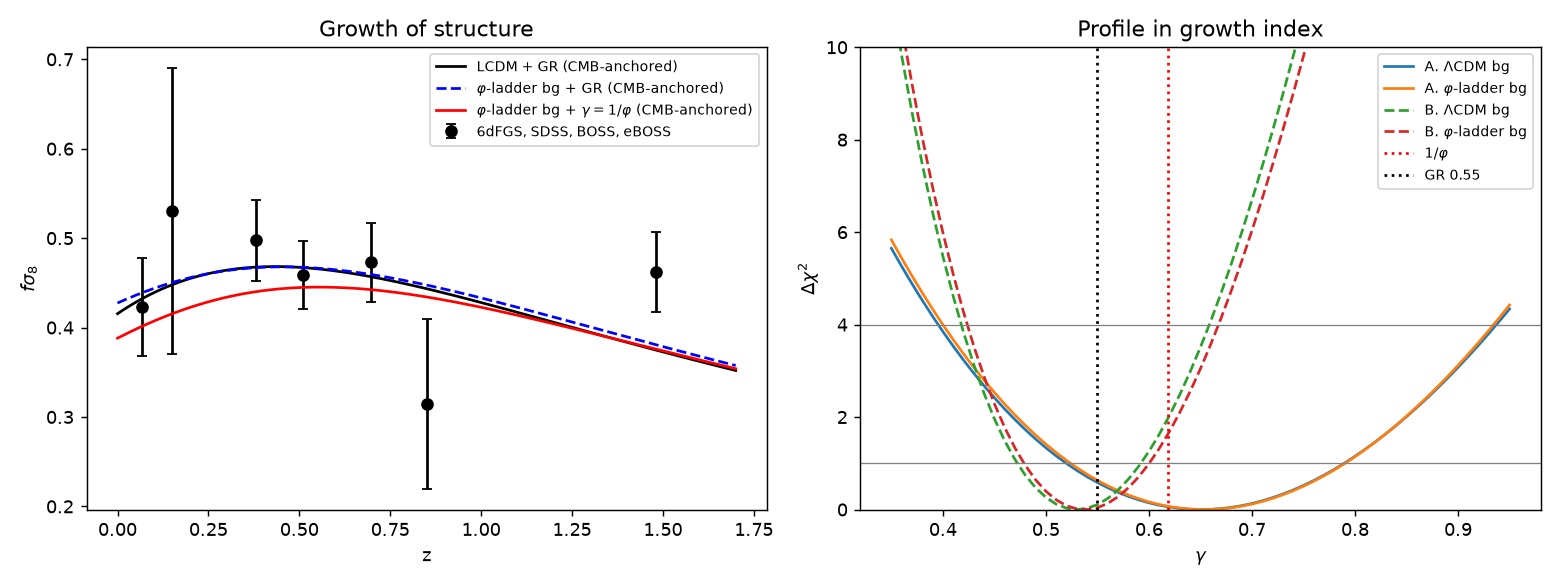
\includegraphics[width=\textwidth]{figures/fig5_growth_index.png}\\[4pt]
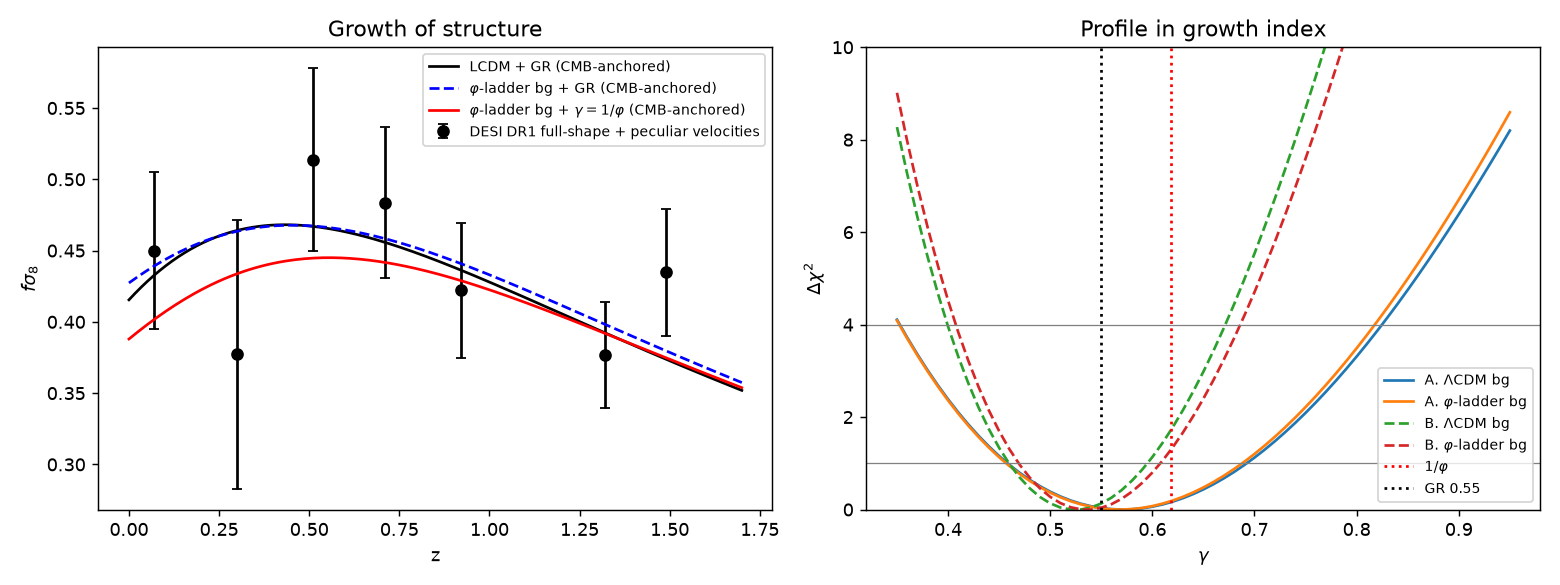
\includegraphics[width=\textwidth]{figures/fig7_growth_index_desi.png}
\caption{Top: SDSS-era $f\sigma_8$ data. Bottom: DESI DR1 full-shape and peculiar-velocity data. Left panels: data and CMB-anchored model curves. Right panels: $\Delta\chi^2$ profile in $\gamma$ for shape-only (solid) and CMB-anchored (dashed) fits.}
\label{fig:growth}
\end{figure}

\subsection{Early dark energy and $H_0$: a corrected claim}

An earlier version of this proposal derived $r_d = 147.09\,(1 - \fede) = 136.36$\,Mpc and hence $H_0 = 67.40/(1-\fede) = 72.70$\,km\,s$^{-1}$\,Mpc$^{-1}$. This assumes that the sound horizon shrinks by exactly the energy fraction, which is incorrect. In the standard fluid approximation to the axion-like early dark energy of Ref.~\cite{Poulin} ($n = 3$, so $w_n = (n-1)/(n+1) = 1/2$):
\begin{itemize}
\item $\fede = 0.073$ reduces $r_d$ by only $0.8$--$2.4\%$ for $z_c = 10^3$--$10^4$ (Fig.~\ref{fig:ede});
\item reaching $136.36$\,Mpc would require $\fede \approx 0.21$;
\item the implied $H_0$ ranges from $69.0$ (holding $H_0 r_d$ fixed) to $76.0$\,km\,s$^{-1}$\,Mpc$^{-1}$ (holding $\theta_*$ and $\omega_c$ fixed), and only a full Boltzmann-code fit can settle it.
\end{itemize}
We therefore \emph{do not} predict $H_0$. Current 95\% upper limits are:
\begin{itemize}
\item $\fede < 0.070$ from Planck CMB and lensing, and $< 0.091$ adding DESI BAO~\cite{EDElim1};
\item $< 0.065$ (Planck NPIPE) and $< 0.092$ (Planck + ACT DR6), both with CMB lensing and Pantheon+ and without DESI BAO or the SH0ES prior; adding DESI DR2 BAO to the second gives $< 0.109$~\cite{Poulin2025};
\item $< 0.12$ for a combination including ACT DR6~\cite{EDElim2}.
\end{itemize}
Prediction~\ref{pred:ede} is therefore already under pressure. Including this early dark energy does not change the agreement of Prediction~\ref{pred:de} with the data (Appendix~\ref{sec:joint}).

\begin{figure}[t]
\centering
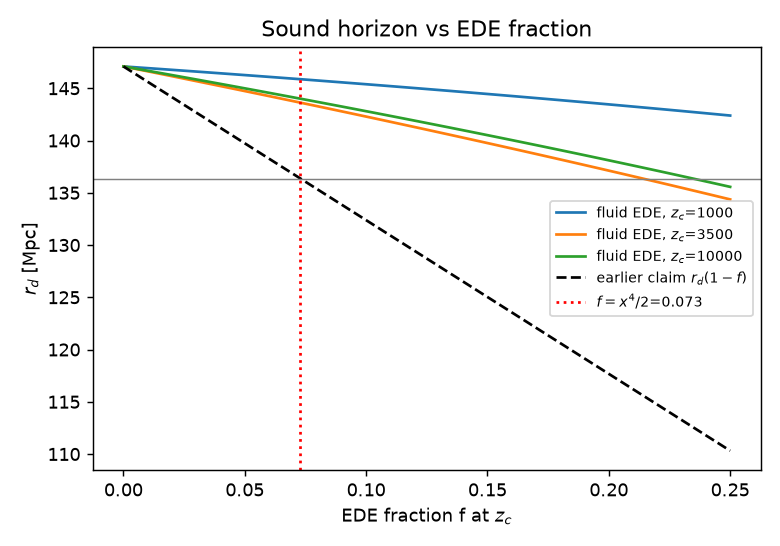
\includegraphics[width=0.6\textwidth]{figures/fig3_ede.png}
\caption{Drag-epoch sound horizon versus peak early-dark-energy fraction for three critical redshifts $z_c$, compared with the incorrect scaling $r_d(1-f)$ (dashed).}
\label{fig:ede}
\end{figure}

%==========================================================================
\section{Pre-registered predictions and falsification criteria}\label{sec:prereg}

The following were time-stamped on \lockdate\ (Zenodo DOI: \href{https://doi.org/10.5281/zenodo.23481070}{10.5281/zenodo.23481070}). The SHA-256 hash of the prediction record is
\begin{center}\footnotesize\texttt{\lockhash}\end{center}

\paragraph{What counts as a test.} DESI's DR2 results use observations from 14 May 2021 to 9 April 2024~\cite{DESI-DR2}, and the predictions were chosen after them. The first DESI test is therefore any cosmology analysis that includes observations made after 9 April 2024. No release date for such results has been announced. Because future DESI analyses also contain the DR2 data, part of their agreement is built in; fully independent tests come from other probes (Euclid growth measurements, new supernova samples and CMB experiments).

\begin{prediction}\label{pred:de}
$(w_0, w_a) = (-\gr/2, -1/\gr) = (-0.80902, -0.61803)$, equivalently $w_a = 1 + 2w_0$ with $w_0 = -\gr/2$. Hence $w = -1$ at $z = 1/\sqrt5$, $w(0.3) = -0.9516$ and $w(0.5) = -1.0150$.

\emph{Falsified} if any of the following holds in the first DESI analysis including post-DR2 data:
\begin{itemize}
\item the point lies outside the $3\sigma$ region ($\Delta\chi^2 > 11.83$) of the $w_0$--$w_a$ constraint from BAO + CMB alone, or from BAO + CMB + SNe for at least two of the principal SN compilations;
\item $w(0.3)$ or $w(0.5)$ differs from the prediction by more than $3\sigma$ in at least two of these combinations.
\end{itemize}

\emph{Supported} if the point stays within $2\sigma$ in all combinations while \LCDM\ is excluded at more than $3\sigma$.
\end{prediction}

\begin{prediction}\label{pred:gamma}
$\gamma = 1/\gr = 0.618$, constant for $0 \le z \le 1$.

\emph{Falsified} by a measurement with $\sigma_\gamma \le 0.03$ lying more than $3\sigma$ from $0.618$.
\end{prediction}

\begin{prediction}\label{pred:ede}
$\fede = \tfrac12 x^4 = (5 - 3\gr)/2 = 0.07295$ (axion-like EDE, $n = 3$, $z_c$ free).

\emph{Falsified} if excluded at 99.7\%.
\end{prediction}

Derived, not independently tested: $S_8 \approx 0.81$ ($0.812$ in the best-fit background of Sec.~\ref{sec:growth}; approximate, because it depends on the background fit). $H_0$ is not predicted.

%==========================================================================
\section{Open problems}\label{sec:open}

\begin{problem}[The bridge]
Sec.~\ref{sec:math} proves that $1/\gr$ characterizes maximal non-resonance. Why the cosmological dark sector should be governed by this property is postulated (Hypothesis~\ref{hyp:1}), not derived.

\emph{A conjectural route.} In the minisuperspace (Hamiltonian) description, a closed Friedmann universe with one scalar field has two degrees of freedom $(a, \phi)$: a four-dimensional phase space on which the Friedmann equation defines a three-dimensional constraint surface, which is exactly the setting of the KAM results of Sec.~\ref{sec:math}. This system is known to be chaotic~\cite{Page84,CalzettaElHasi,CornishShellard}. For a spatially flat universe with a single field, the dynamics reduces to the two-dimensional autonomous system $(\phi, \dot\phi)$, which cannot be chaotic. However, a single canonical scalar field cannot cross $w = -1$~\cite{Vikman}; the simplest models that do, quintom models, use two fields~\cite{QuintomReview}, and two-field cosmological dynamics can be chaotic~\cite{EastherMaeda}. We therefore conjecture that the dynamics of a (multi-field) dark sector is organized by its most robust non-resonant barriers, the golden ones. Showing this, and showing that it produces the ladder of Hypothesis~\ref{hyp:2}, is open. In particular, why the early-dark-energy fraction should be a $d = 4$ term is not explained.
\end{problem}

\begin{problem}[The ladder]
The weights $\alpha_d$ and the assignment of $d$ to each observable (Hypotheses~\ref{hyp:2} and~\ref{hyp:3}) are postulates. The rival $d = 3$ branch ($w_0 = -0.764$) fits worse but is not excluded by any principle.
\end{problem}

\begin{problem}[The value of $w_a$]\label{op:wa}
$w_a = -1/\gr$, or equivalently the crossing position $1 - a_{\rm cross} = x/2$, is postulated, not derived. A dynamical model that yields both $w_0$ and $w_a$ from one equation of motion is needed.
\end{problem}

\begin{problem}[Mechanism]\label{op:mech}
The effective embedding of Sec.~\ref{sec:embed}, PPF dark energy plus $\mu_0 \simeq -0.20$, is consistent but phenomenological. It also leaves the lensing response $\Sigma$ open; current data require $\Sigma_0 \approx 0$ to within about $0.05$~\cite{Ishak}. Pure momentum exchange cannot produce the growth suppression across the crossing (Appendix~\ref{sec:drag}). A candidate is energy exchange,
\begin{equation}
\dot\rho_c + 3H\rho_c = -Q, \qquad \dot\rho_{\rm DE} + 3H(1+w)\rho_{\rm DE} = +Q.
\end{equation}
An observer who assumes $\rho_c \propto a^{-3}$ infers $\rho_{\rm DE,eff} = \rho_{\rm DE} + \Delta$, with $\Delta = \rho_c - \rho_{c,0}a^{-3}$, and
\begin{equation}
1 + w_{\rm eff} = \frac{(1+w)\,\rho_{\rm DE} + \Delta}{\rho_{\rm DE} + \Delta}.
\end{equation}
An apparent phantom past ($w_{\rm eff} < -1$) therefore needs $\Delta < 0$: dark matter must have been less dense in the past than $a^{-3}$ implies, so energy must flow \emph{from dark energy to dark matter} ($Q < 0$)~\cite{DasCorasanitiKhoury}.

We tested the simplest forms, $Q = -\xi H\rho_{\rm DE}$ and $Q = -\xi H\rho_c$, with constant $w = -\gr/2$, at the level of the background:
\begin{itemize}
\item The crossing can be placed at $z = 1/\sqrt5$, with $\xi = 0.34$ and $0.58$ respectively, and $w_{\rm eff}$ then follows the prediction to within $0.04$ up to $z = 0.5$.
\item Beyond that, $w_{\rm eff}$ falls far too fast ($-1.73$ and $-2.00$ at $z = 1$, against $-1.12$ predicted), and the inferred dark-energy density turns negative by $z = 1.6$ and $1.4$.
\end{itemize}
These simple forms are therefore excluded as the mechanism. A viable model would need a time-dependent coupling or equation of state, and its growth rate ($\mu_0$) depends on how momentum is transferred, which we have not modeled.
\end{problem}

\begin{problem}[Beyond cosmology]
The intuition that recursive, non-resonant partitioning of phase space also organizes protein folding or neural action selection is not expressed here as a quantitative prediction, and is not claimed. Any such claim would need to compete with established explanations:
\begin{itemize}
\item \textbf{Protein folding.} Energy-landscape (``folding funnel'') theory resolves Levinthal's paradox with biased, multi-pathway search~\cite{DillChan}.
\item \textbf{Readiness potential.} The pre-movement potential has been modeled as the accumulation of ongoing neural noise rather than a pre-made decision~\cite{Schurger}.
\end{itemize}
A testable version would have to predict, for example, folding-time scaling or readiness-potential timing.
\end{problem}

%==========================================================================
\section{Conclusion}

We have reduced an intuition, that trajectories in higher-dimensional phase space must avoid one another and that this organizes nature around the golden ratio, to two separate parts:
\begin{itemize}
\item \textbf{Mathematics:} proven results (non-merging of distinct states; $1/\gr$ as the global attractor of recursive self-similar partitioning and the most non-resonant number), plus well-supported numerical evidence that golden tori are the most robust KAM barriers.
\item \textbf{A falsifiable hypothesis:} the dark-sector parameters that differ from \LCDM\ take ladder values $\alpha_d x^d$.
\end{itemize}

The hypothesis fixes $w_0 = -\gr/2$ and $w_a = -1/\gr$ without free parameters. With compressed CMB information this pair lies $0.3$--$1.0\sigma$ from the best free fit, including the recalibrated DES-Dovekie sample, and has the lowest AIC and BIC in every combination. In DESI's official posteriors it lies at $0.5$--$1.0\sigma$ when supernovae are included, and it is robust to the choice of CMB likelihood. It is the only member of its 403-member algebraic family within $1\sigma$ of all three supernova samples. The agreement does not depend on the CMB or on the predicted early dark energy, and the full predicted $w(z)$ matches DESI's binned reconstruction about as well as DESI's own best-fit model.

When $x$ is fitted freely, the data give $x \approx 0.55$--$0.69$, consistent with $1/\gr$ but unable to single it out. The fixed-point Bayes factors favor a simple point near $1/\gr$ over free $(w_0, w_a)$ and over \LCDM, but not $\gr$ specifically.

Each prediction has an established effective form: PPF dark energy for the crossing, $\mu_0 \simeq -0.20$ for growth, and axion-like early dark energy. The status of the other claims:
\begin{itemize}
\item The growth index $1/\gr$ is mildly disfavored, at about $1\sigma$, by two independent $f\sigma_8$ data sets.
\item The early-dark-energy fraction is in tension with some CMB limits.
\item An earlier $H_0$ claim is withdrawn.
\item Neither momentum exchange nor the simplest energy-exchange couplings can reproduce the predicted growth suppression and $w(z)$ together.
\end{itemize}

The predictions are time-stamped. DESI data beyond DR2, Euclid and next-generation CMB experiments will decide them.

\section*{Data and code availability}
All analysis code and outputs are archived on Zenodo (DOI \href{https://doi.org/10.5281/zenodo.23481070}{10.5281/zenodo.23481070}) and on GitHub (\url{https://github.com/letsbuild9/golden-ratio-dark-energy}):
{\raggedright
\begin{itemize}
\item likelihoods, fits and validation: \texttt{borse\_fit.py}, \texttt{borse\_calibrate\_zstar.py}, \texttt{borse\_checks.py} and \texttt{borse\_camb\_check.py};
\item official DESI chains and robustness tests: \texttt{borse\_desi\_chains.py}, \texttt{borse\_v2\_tests.py}, \texttt{borse\_v2b\_tests.py} and \texttt{borse\_binned\_calibration.py};
\item growth and mechanism tests: \texttt{borse\_growth.py}, \texttt{borse\_mu.py}, \texttt{borse\_model.py} and \texttt{borse\_energy\_exchange.py};
\item verification: \texttt{borse\_symbolic.py} (exact symbolic proofs), \texttt{verify\_paper.py} (an automated check that every number quoted here matches the outputs) and a ledger recording the source of every external value;
\item \texttt{lock\_predictions.py}, which writes the time-stamped prediction record and its hash.
\end{itemize}
\par}
Public data were obtained from:
\begin{itemize}
\item the DESI DR2 BAO cosmology chain release~\cite{DESIchains};
\item the DESI DR1 full-shape~\cite{DESI-FS} and peculiar-velocity~\cite{DESI-PV} analyses;
\item SDSS DR16~\cite{eBOSS};
\item the Pantheon+, Union3, DES-SN5YR and DES-Dovekie releases, via the Cobaya \texttt{bao\_data} and \texttt{sn\_data} repositories.
\end{itemize}

\section*{Acknowledgements}
\textbf{Use of AI tools.} The original framework was developed in conversations with an AI system (Gemini, Google), which also produced several claims later found to be incorrect and withdrawn here. Numerical analysis, verification and drafting were assisted by an AI system (Claude, Anthropic). The author is responsible for all content.

\textbf{DESI.} This research used data obtained with the Dark Energy Spectroscopic Instrument (DESI). DESI construction and operations is managed by the Lawrence Berkeley National Laboratory. This material is based upon work supported by the U.S. Department of Energy, Office of Science, Office of High-Energy Physics, under Contract No.\ DE--AC02--05CH11231, and by the National Energy Research Scientific Computing Center, a DOE Office of Science User Facility under the same contract. Additional support for DESI was provided by the U.S. National Science Foundation (NSF), Division of Astronomical Sciences under Contract No.\ AST-0950945 to the NSF's National Optical-Infrared Astronomy Research Laboratory; the Science and Technology Facilities Council of the United Kingdom; the Gordon and Betty Moore Foundation; the Heising-Simons Foundation; the French Alternative Energies and Atomic Energy Commission (CEA); the National Council of Humanities, Science and Technology of Mexico (CONAHCYT); the Ministry of Science and Innovation of Spain (MICINN), and by the DESI Member Institutions: \url{www.desi.lbl.gov/collaborating-institutions}. The DESI collaboration is honored to be permitted to conduct scientific research on I'oligam Du'ag (Kitt Peak), a mountain with particular significance to the Tohono O'odham Nation. Any opinions, findings, and conclusions or recommendations expressed in this material are those of the author(s) and do not necessarily reflect the views of the U.S. National Science Foundation, the U.S. Department of Energy, or any of the listed funding agencies.

\textbf{SDSS.} Funding for the Sloan Digital Sky Survey IV has been provided by the Alfred P. Sloan Foundation, the U.S. Department of Energy Office of Science, and the Participating Institutions. SDSS-IV acknowledges support and resources from the Center for High Performance Computing at the University of Utah. The SDSS website is \url{www.sdss4.org}. SDSS-IV is managed by the Astrophysical Research Consortium for the Participating Institutions of the SDSS Collaboration including the Brazilian Participation Group, the Carnegie Institution for Science, Carnegie Mellon University, Center for Astrophysics \textbar{} Harvard \& Smithsonian, the Chilean Participation Group, the French Participation Group, Instituto de Astrof\'{\i}sica de Canarias, The Johns Hopkins University, Kavli Institute for the Physics and Mathematics of the Universe (IPMU) / University of Tokyo, the Korean Participation Group, Lawrence Berkeley National Laboratory, Leibniz Institut f\"ur Astrophysik Potsdam (AIP), Max-Planck-Institut f\"ur Astronomie (MPIA Heidelberg), Max-Planck-Institut f\"ur Astrophysik (MPA Garching), Max-Planck-Institut f\"ur Extraterrestrische Physik (MPE), National Astronomical Observatories of China, New Mexico State University, New York University, University of Notre Dame, Observat\'ario Nacional / MCTI, The Ohio State University, Pennsylvania State University, Shanghai Astronomical Observatory, United Kingdom Participation Group, Universidad Nacional Aut\'onoma de M\'exico, University of Arizona, University of Colorado Boulder, University of Oxford, University of Portsmouth, University of Utah, University of Virginia, University of Washington, University of Wisconsin, Vanderbilt University, and Yale University.

\textbf{Planck.} Based on observations obtained with Planck (\url{http://www.esa.int/Planck}), an ESA science mission with instruments and contributions directly funded by ESA Member States, NASA, and Canada.

%==========================================================================
\appendix

\section{Model-independent shape: DESI's binned $w(z)$}\label{sec:binned}

CPL is only a local parametrization. DESI also fits $w$ as piecewise constant in $z = 0$--$0.7$, $0.7$--$1.4$, $1.4$--$2.1$ and $2.1$--$10$, with $w = -1$ beyond~\cite{DESIchains}. DESI's implementation smooths the steps between bins (fixed smoothing parameter $s = 0.02$ in the released configuration); we treat the bins as sharp. We compare the official binned posteriors with the predicted $w(z)$ averaged over each bin, uniformly in $z$ (Table~\ref{tab:binned}). Uniform averaging is only an approximation to what a piecewise-constant fit returns, so we calibrate it by applying the identical averaging to each data set's own $w_0w_a$CDM posterior-mean model.

\begin{table}[h]
\centering
\small
\begin{tabular}{lccccc}
\toprule
Official binned chains & $w$ ($0$--$0.7$) & $w$ ($0.7$--$1.4$) & $w$ ($1.4$--$2.1$) & $\gr$-ladder & DESI's CPL \\
\midrule
DESI+CMB & $-0.840 \pm 0.073$ & $-1.485 \pm 0.204$ & $-1.209 \pm 0.772$ & $1.18\sigma$ & $0.29\sigma$ \\
+Pantheon+ & $-0.919 \pm 0.030$ & $-1.384 \pm 0.172$ & $-1.255 \pm 0.751$ & $1.01\sigma$ & $1.53\sigma$ \\
+Union3 & $-0.862 \pm 0.042$ & $-1.454 \pm 0.181$ & $-1.209 \pm 0.753$ & $1.75\sigma$ & $0.91\sigma$ \\
+DESY5 & $-0.894 \pm 0.029$ & $-1.362 \pm 0.168$ & $-1.366 \pm 0.746$ & $1.63\sigma$ & $1.52\sigma$ \\
\bottomrule
\end{tabular}
\caption{DESI DR2 binned $w(z)$ versus bin-averaged predictions; the predicted averages are $-0.959$, $-1.123$ and $-1.201$. The last two columns give the joint deviation over the first three bins (full covariance, 3 degrees of freedom) for the $\gr$-ladder and for each data set's own CPL posterior-mean model.}
\label{tab:binned}
\end{table}

The predicted $w(z)$ is consistent with the binned reconstruction at $1.0$--$1.75\sigma$, comparable to DESI's own best-fit CPL models ($0.3$--$1.5\sigma$). Both CPL curves are less negative than the data between $z = 0.7$ and $1.4$ and, except for DESI's own fit to DESI+CMB, more negative below $z = 0.7$. This appears to be a limitation of the CPL shape rather than of the golden-ratio values.

\section{Joint check: dark energy with the predicted early dark energy}\label{sec:joint}

The dark-energy fits of Sec.~\ref{sec:tests} assume standard early physics, but the hypothesis also predicts $\fede = 0.073$, which shortens the sound horizon. We test whether Prediction~\ref{pred:de} survives this in two ways.

\textbf{(a) Independent of early physics.} DESI BAO alone, or with each SN sample, with $r_d$ left free (only $h\,r_d$ enters, so any early-universe change is absorbed) and no CMB. The $\gr$-ladder lies $1.07$ (BAO only), $0.76$ (+Pantheon+), $0.63$ (+Union3), $0.10$ (+DESY5) and $0.25\sigma$ (+DES-Dovekie) from the free fit, while \LCDM\ is disfavored at $1.7$--$3.3\sigma$. This agrees with the official no-CMB chains of Table~\ref{tab:official}.

\textbf{(b) With CMB and early dark energy (indicative).} We add the axion-like fluid with $\fede = 0.073$ to $H(z)$ for $z_c = 10^3$, $3.5\times10^3$ and $10^4$, and rescale $r_d$ and $r_s(z_*)$ by the ratio of the sound-horizon integrals with and without it ($r_d$ shrinks by $0.8$--$2.3\%$). Across all $z_c$ and data combinations the $\gr$-ladder stays $0.2$--$1.3\sigma$ from the free fit, \LCDM\ is disfavored at $2.0$--$4.0\sigma$, and $H_0$ rises to $68.1$--$70.4$\,km\,s$^{-1}$\,Mpc$^{-1}$. The compressed CMB priors assume standard early physics, so this case is indicative only; a full Boltzmann-code analysis with the CMB likelihood is needed for a definitive statement.

\textbf{Conclusion.} At current precision, Prediction~\ref{pred:de} does not depend on whether the predicted early dark energy is present.

\section{Momentum exchange as the growth mechanism: a negative result}\label{sec:drag}

A natural mechanism for suppressing growth without altering the background is elastic dark-matter--dark-energy scattering~\cite{Simpson}, related to the pure-momentum-transfer coupling of Pourtsidou, Skordis \& Copeland~\cite{PSC}. In the sub-horizon, quasi-static limit, with $N = \ln a$,
\begin{align}
\delta_c'' + \left(2 + \frac{\mathrm d\ln H}{\mathrm dN} + \xi\,(1+w)\,\Omega_{\rm DE}\frac{H}{H_0}\right)\delta_c' &= \tfrac32\left(\Omega_c\delta_c + \Omega_b\delta_b\right),\\
\delta_b'' + \left(2 + \frac{\mathrm d\ln H}{\mathrm dN}\right)\delta_b' &= \tfrac32\left(\Omega_c\delta_c + \Omega_b\delta_b\right),
\end{align}
with $\xi = (\sigma_D/m_c)\,c\,\rho_{\rm crit,0}/H_0$. Because the drag is proportional to $1 + w$, it \emph{reverses sign} above $z_{\rm cross}$. Integrating in the $\gr$-ladder background (Fig.~\ref{fig:drag}), with a target suppression equal to that implied by $\gamma = 1/\gr$ (Prediction~\ref{pred:gamma}), i.e.\ $\gamma - \gamma_{\rm GR} \approx 0.06$--$0.08$ for $0 \le z \le 1.5$:
\begin{itemize}
\item \textbf{No coupling $\xi \ge 0$ produces the required suppression.} The target is a 2.6\% lower growth factor at $z = 0$. Instead, growth is \emph{enhanced}, by $+0.45\%$ for $\xi = (7\gr - 10)/4 \approx 0.33$ and by $+4.2\%$ for $\xi = 3$.
\item \textbf{A non-crossing history fixes the sign but is excluded.} A CPL history with the same $w_0$ never crosses $-1$ only if $w_a \ge -(1+w_0) = -0.191$. At this boundary a coupling $\xi \approx 2.3$ ($\sigma_D/m_c \approx 36$\,b/GeV) gives an almost constant $\Delta\gamma = 0.066$--$0.072$ for $0 \le z \le 1.5$, close to the $0.059$--$0.069$ required in that background. However, this history is excluded at $4.2$--$4.9\sigma$ by the data of Table~\ref{tab:fits}, and at $4.0$--$5.3\sigma$ (Gaussian estimate) in the official DESI posteriors.
\end{itemize}
Momentum exchange can therefore produce the growth suppression only in a background that the data exclude.

\begin{figure}[t]
\centering
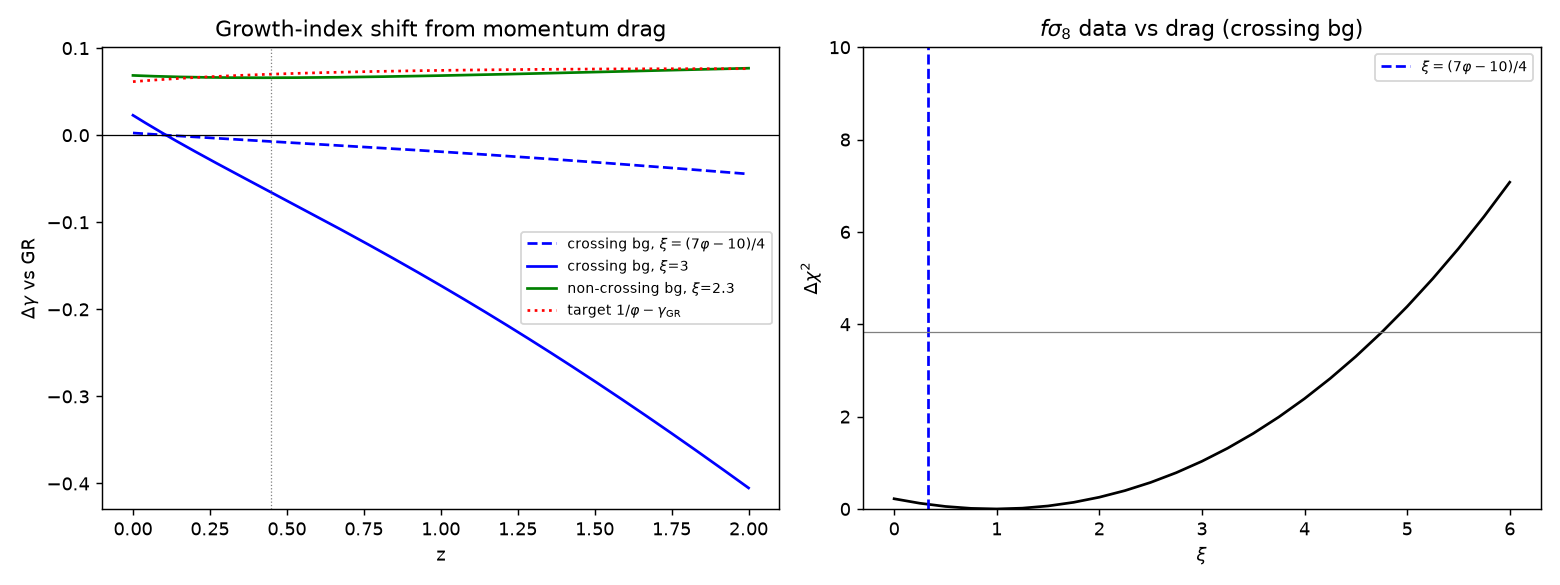
\includegraphics[width=\textwidth]{figures/fig6_drag_model.png}
\caption{Left: growth-index shift produced by dark-matter--dark-energy momentum exchange. Blue: phantom-crossing $\gr$-ladder background. Green: non-crossing background. Dotted red: target, $1/\gr - \gamma_{\rm GR}(z)$. Right: $f\sigma_8$ constraint on $\xi$ in the crossing background.}
\label{fig:drag}
\end{figure}

%==========================================================================
\begin{thebibliography}{99}\small\raggedright
\bibitem{DESI-DR2} DESI Collaboration, \emph{DESI DR2 Results II: Measurements of Baryon Acoustic Oscillations and Cosmological Constraints}, Phys.\ Rev.\ D 112, 083515 (2025), arXiv:2503.14738.
\bibitem{DESI-Y1} DESI Collaboration, \emph{DESI 2024 VI: Cosmological Constraints from the Measurements of Baryon Acoustic Oscillations}, JCAP 02 (2025) 021, arXiv:2404.03002.
\bibitem{DESIchains} DESI Collaboration, \emph{DESI DR2 BAO cosmology results} (chains and best fits), \url{https://data.desi.lbl.gov/public/papers/y3/bao-cosmo-params} (released October 2025).
\bibitem{Dovekie} B.~Popovic et al., \emph{The Dark Energy Survey Supernova Program: A Reanalysis of Cosmology Results and Evidence for Evolving Dark Energy}, MNRAS (2026), arXiv:2511.07517.
\bibitem{Planck2018} Planck Collaboration (N.~Aghanim et al.), \emph{Planck 2018 results. VI. Cosmological parameters}, A\&A 641, A6 (2020), arXiv:1807.06209.
\bibitem{DESY3} DES Collaboration (T.~M.~C.~Abbott et al.), \emph{Dark Energy Survey Year 3 results: Cosmological constraints from galaxy clustering and weak lensing}, Phys.\ Rev.\ D 105, 023520 (2022), arXiv:2105.13549.
\bibitem{KiDSLegacy} A.~H.~Wright et al., \emph{KiDS-Legacy: Cosmological constraints from cosmic shear with the complete Kilo-Degree Survey}, A\&A 703, A158 (2025), arXiv:2503.19441.
\bibitem{SH0ES} A.~G.~Riess et al., ApJL 934, L7 (2022), doi:10.3847/2041-8213/ac5c5b.
\bibitem{CruzGolden} N.~Cruz, M.~Olivares and J.~R.~Villanueva, \emph{The golden ratio in Schwarzschild--Kottler black holes}, arXiv:1701.03166 (2017).
\bibitem{BryantHobill} M.~S.~Bryant and D.~W.~Hobill, \emph{Bianchi IX Cosmologies and the Golden Ratio}, arXiv:1610.04223 (2016).
\bibitem{ArnoldODE} V.~I.~Arnold, \emph{Ordinary Differential Equations} (Springer, 1992); \emph{Mathematical Methods of Classical Mechanics}, 2nd ed.\ (Springer, 1989).
\bibitem{Sakurai} J.~J.~Sakurai and J.~Napolitano, \emph{Modern Quantum Mechanics}, 3rd ed.\ (Cambridge University Press, 2020).
\bibitem{Hurwitz} A.~Hurwitz, \emph{Ueber die angen\"aherte Darstellung der Irrationalzahlen durch rationale Br\"uche}, Math.\ Ann.\ 39, 279--284 (1891), doi:10.1007/BF01206656.
\bibitem{Kolmogorov} A.~N.~Kolmogorov, Dokl.\ Akad.\ Nauk SSSR 98, 527 (1954).
\bibitem{Arnold63} V.~I.~Arnold, Russ.\ Math.\ Surveys 18(5), 9--36 (1963), doi:10.1070/RM1963v018n05ABEH004130.
\bibitem{Moser} J.~Moser, Nachr.\ Akad.\ Wiss.\ G\"ottingen II, 1 (1962).
\bibitem{Greene} J.~M.~Greene, \emph{A method for determining a stochastic transition}, J.\ Math.\ Phys.\ 20, 1183--1201 (1979), doi:10.1063/1.524170.
\bibitem{MacKay} R.~S.~MacKay, \emph{A renormalisation approach to invariant circles in area-preserving maps}, Physica D 7, 283--300 (1983), doi:10.1016/0167-2789(83)90131-8.
\bibitem{ArnoldDiffusion} V.~I.~Arnold, \emph{Instability of dynamical systems with several degrees of freedom}, Sov.\ Math.\ Dokl.\ 5, 581 (1964).
\bibitem{CPL1} M.~Chevallier and D.~Polarski, Int.\ J.\ Mod.\ Phys.\ D 10, 213--223 (2001), doi:10.1142/S0218271801000822.
\bibitem{CPL2} E.~V.~Linder, Phys.\ Rev.\ Lett.\ 90, 091301 (2003), doi:10.1103/PhysRevLett.90.091301.
\bibitem{QuintomReview} T.-t.~Qiu, Y.-F.~Cai et al., \emph{A Focused Review of Quintom Cosmology: From Quintom Dark Energy to Quintom Bounce}, arXiv:2511.19994 (2025).
\bibitem{WangSteinhardt} L.~Wang and P.~J.~Steinhardt, ApJ 508, 483--490 (1998), doi:10.1086/306436.
\bibitem{Linder05} E.~V.~Linder, Phys.\ Rev.\ D 72, 043529 (2005), doi:10.1103/PhysRevD.72.043529.
\bibitem{Vikman} A.~Vikman, \emph{Can dark energy evolve to the phantom?}, Phys.\ Rev.\ D 71, 023515 (2005).
\bibitem{FangHuLewis} W.~Fang, W.~Hu and A.~Lewis, \emph{Crossing the phantom divide with parameterized post-Friedmann dark energy}, Phys.\ Rev.\ D 78, 087303 (2008).
\bibitem{AKS} L.~Amendola, M.~Kunz and D.~Sapone, \emph{Measuring the dark side (with weak lensing)}, JCAP 04, 013 (2008).
\bibitem{Ishak} M.~Ishak et al.\ (DESI Collaboration), \emph{Modified Gravity Constraints from the Full Shape Modeling of Clustering Measurements from DESI 2024}, JCAP 09 (2025) 053, arXiv:2411.12026.
\bibitem{Poulin} V.~Poulin, T.~L.~Smith, T.~Karwal and M.~Kamionkowski, \emph{Early Dark Energy Can Resolve The Hubble Tension}, Phys.\ Rev.\ Lett.\ 122, 221301 (2019).
\bibitem{ChenHuangWang} L.~Chen, Q.-G.~Huang and K.~Wang, \emph{Distance Priors from Planck Final Release}, arXiv:1808.05724.
\bibitem{PantheonPlus} D.~Brout et al., \emph{The Pantheon+ Analysis: Cosmological Constraints}, ApJ 938, 110 (2022), arXiv:2202.04077.
\bibitem{Union3} D.~Rubin et al., \emph{Union Through UNITY: Cosmology with 2,000 SNe Using a Unified Bayesian Framework}, arXiv:2311.12098 (2023).
\bibitem{DESY5} DES Collaboration, \emph{The Dark Energy Survey: Cosmology Results with $\sim$1500 New High-redshift Type Ia Supernovae}, ApJL 973, L14 (2024), arXiv:2401.02929.
\bibitem{Komatsu} E.~Komatsu et al., \emph{Seven-Year WMAP Observations: Cosmological Interpretation}, ApJS 192, 18 (2011), eq.~26.
\bibitem{HuSugiyama} W.~Hu and N.~Sugiyama, ApJ 471, 542--570 (1996), doi:10.1086/177989.
\bibitem{CAMB} A.~Lewis, A.~Challinor and A.~Lasenby, \emph{Efficient computation of CMB anisotropies in closed FRW models}, ApJ 538, 473--476 (2000).
\bibitem{6dF} F.~Beutler et al., MNRAS 423, 3430--3444 (2012), doi:10.1111/j.1365-2966.2012.21136.x.
\bibitem{MGS} C.~Howlett et al., MNRAS 449, 848--866 (2015), doi:10.1093/mnras/stu2693.
\bibitem{eBOSS} eBOSS Collaboration (S.~Alam et al.), Phys.\ Rev.\ D 103, 083533 (2021), arXiv:2007.08991.
\bibitem{DESI-FS} DESI Collaboration (A.~G.~Adame et al.), \emph{DESI 2024 V: Full-Shape Galaxy Clustering from Galaxies and Quasars}, JCAP 09 (2025) 008, arXiv:2411.12021.
\bibitem{DESI-PV} R.~J.~Turner et al., \emph{The DESI DR1 Peculiar Velocity Survey: growth rate measurements from galaxy and momentum correlation functions}, arXiv:2512.03230.
\bibitem{LyaFS} M.~Herbold et al., \emph{Validation of the DESI DR2 Ly$\alpha$ forest full-shape analysis}, arXiv:2607.27411 (2026).
\bibitem{Nguyen} N.-M.~Nguyen, D.~Huterer and Y.~Wen, \emph{Evidence for suppression of structure growth in the concordance cosmological model}, Phys.\ Rev.\ Lett.\ 131, 111001 (2023).
\bibitem{Simpson} F.~Simpson, \emph{Scattering of dark matter and dark energy}, Phys.\ Rev.\ D 82, 083505 (2010), arXiv:1007.1034.
\bibitem{PSC} A.~Pourtsidou, C.~Skordis and E.~J.~Copeland, \emph{Models of dark matter coupled to dark energy}, Phys.\ Rev.\ D 88, 083505 (2013), arXiv:1307.0458.
\bibitem{EDElim1} F.~J.~Qu et al., \emph{Accelerated inference on accelerated cosmic expansion: New constraints on axion-like early dark energy with DESI BAO and ACT DR6 CMB lensing}, arXiv:2404.16805 (2024).
\bibitem{Poulin2025} V.~Poulin, T.~L.~Smith, R.~Calder\'on and T.~Simon, \emph{Impact of ACT DR6 and DESI DR2 for Early Dark Energy and the Hubble tension}, arXiv:2505.08051 (2025).
\bibitem{EDElim2} A.~Reeves et al., \emph{Multiprobe constraints on early and late time dark energy}, arXiv:2510.06114 (2025).
\bibitem{Page84} D.~N.~Page, \emph{A fractal set of perpetually bouncing universes?}, Class.\ Quantum Grav.\ 1, 417--427 (1984), doi:10.1088/0264-9381/1/4/015.
\bibitem{CalzettaElHasi} E.~Calzetta and C.~El Hasi, \emph{Chaotic Friedmann--Robertson--Walker cosmology}, Class.\ Quantum Grav.\ 10, 1825--1841 (1993), doi:10.1088/0264-9381/10/9/022.
\bibitem{CornishShellard} N.~J.~Cornish and E.~P.~S.~Shellard, \emph{Chaos in quantum cosmology}, Phys.\ Rev.\ Lett.\ 81, 3571--3574 (1998), doi:10.1103/PhysRevLett.81.3571.
\bibitem{EastherMaeda} R.~Easther and K.~Maeda, \emph{Chaotic dynamics and two-field inflation}, Class.\ Quantum Grav.\ 16, 1637--1652 (1999), doi:10.1088/0264-9381/16/5/313.
\bibitem{DasCorasanitiKhoury} S.~Das, P.~S.~Corasaniti and J.~Khoury, \emph{Super-acceleration as signature of dark sector interaction}, Phys.\ Rev.\ D 73, 083509 (2006), arXiv:astro-ph/0510628.
\bibitem{DillChan} K.~A.~Dill and H.~S.~Chan, \emph{From Levinthal to pathways to funnels}, Nat.\ Struct.\ Biol.\ 4, 10--19 (1997), doi:10.1038/nsb0197-10.
\bibitem{Schurger} A.~Schurger, J.~D.~Sitt and S.~Dehaene, \emph{An accumulator model for spontaneous neural activity prior to self-initiated movement}, PNAS 109 (2012), doi:10.1073/pnas.1210467109.
\end{thebibliography}

\end{document}
